% !Mode:: "TeX:UTF-8:Hard"
\documentclass[UTF8]{ctexart}
\usepackage[final]{pdfpages}
\usepackage{amsmath}
\usepackage{mathtools}
\usepackage{geometry}
\usepackage{bm}
\usepackage{amssymb}
\geometry{a4paper,left=3cm,right=3cm}
\newtheorem{thm}{定理}
\newtheorem{define}{定义}

\title{群论考试试题}
\author{艾鑫}


\begin{document}
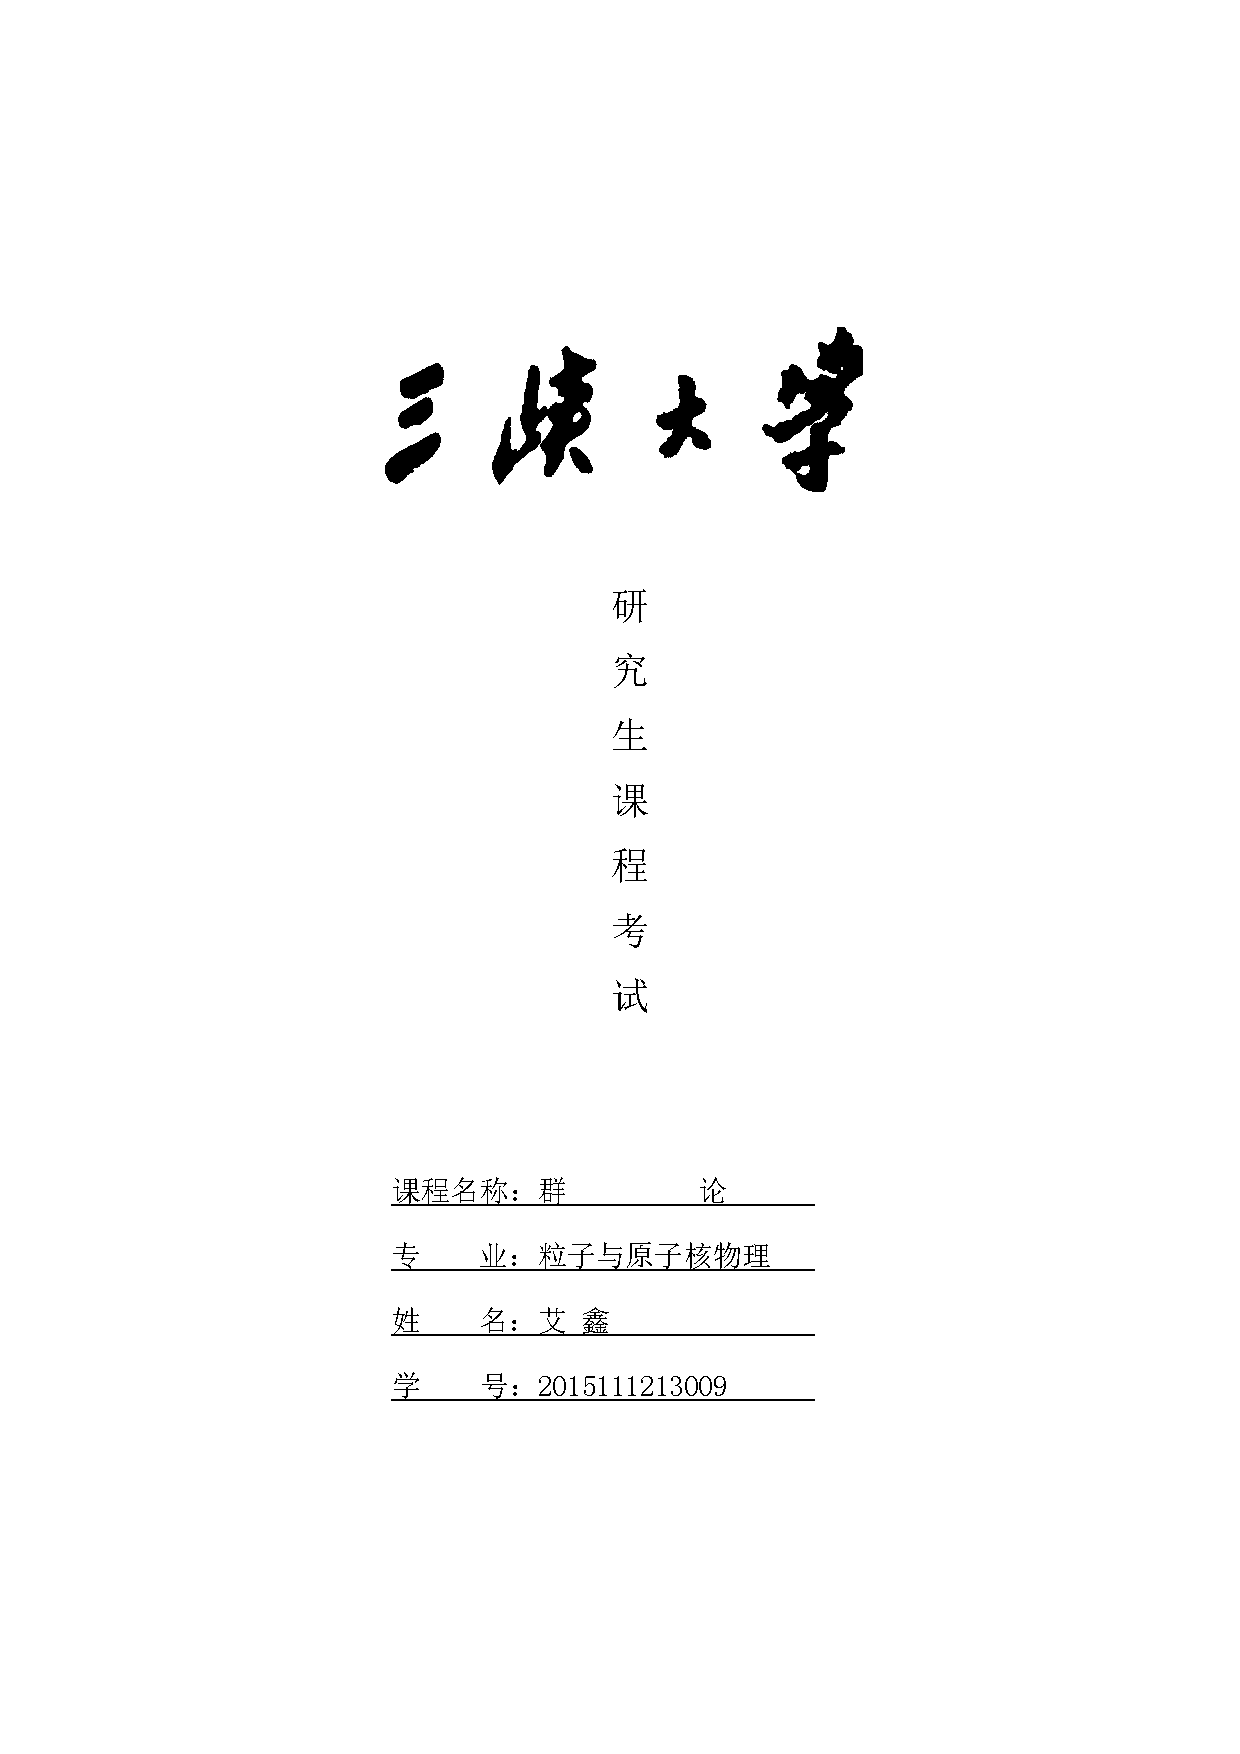
\includepdf{cover.pdf}
\maketitle
\section{有限群:非循环六阶群$G_6^2$}
六阶群有两种结构,其中一个是循环群
\begin{equation}
G_6^1 = \{a,a^2,a^3,a^4,a^5,a^6=e\}
\end{equation}
另外一个就是非循环六阶群$G_6^2 = \{e,a,b,c,d,f\}$,它是最小的非阿贝尔群. 其满足下列关系
\begin{equation}
a^2=b^2=c^2=e, \quad d^2 = f, \quad f^2 = d, \quad fd = df = e
\end{equation}
$G_6^2$的乘法表如下:
\begin{equation}
\begin{array}{|c|c|c|c|c|c|c|}
\hline
G_6^2 & e & a & b & c & d & f \\
\hline
e & e & a & b & c & d & f \\
\hline
a & a & e & d & f & b & c \\
\hline
b & b & f & e & d & c & a \\
\hline
c & c & d & f & e & a & b \\
\hline
d & d & c & a & b & f & e \\
\hline
f & f & b & c & a & e & d \\
\hline
\end{array}
\end{equation}
\subsection{$G_6^2$的构造}

$G_6^2$可以通过保持正三角形不变的所有转动对称变换构成,也就是点群$D_3$.正三角形一共有6个对称操作:
\begin{itemize}
   \item $e$ 恒等变换
   \item $c_3^1$,$c_3^2$分别绕中心点$O$逆时针旋转$2\pi/3$和$4\pi/3$角
   \item $c_{2x}$,$c_{2y}$,$c_{2z}$分别绕$x$,$y$,$z$轴旋转$\pi$角
\end{itemize}
在这种构造中,$c_{2x}$,$c_{2y}$,$c_{2z}$对应于$a$,$b$,$c$;$c_3^1$,$c_3^2$对应于$d$,$f$.

$G_6^2$还可以通过置换群$S_3$来构造。置换群的群元有:
\begin{gather}
\begin{pmatrix}
123 \\
123
\end{pmatrix} = e, \quad
\begin{pmatrix}
123 \\
213
\end{pmatrix} = (12), \quad
\begin{pmatrix}
123 \\
132
\end{pmatrix} = (23) \\
\begin{pmatrix}
123 \\
321
\end{pmatrix} = (31), \quad
\begin{pmatrix}
123 \\
231
\end{pmatrix} = (123), \quad
\begin{pmatrix}
123 \\
312
\end{pmatrix} = (132)
\end{gather}
其中$(12),(23),(31)$对应于$a,b,c$; $(123),(132)$对应于$d,f$.

\subsection{$G_6^2$的子群}
\begin{define}[子群]
群$G$的子集$H$如果在和群$G$相同的乘法规则下也构成群, 则称$H$为群$G$的子群.
\end{define}

对于任意一个群$G$,群$\{e\}$和群$G$本身一定是$G$的子群. 其他的子群, 叫做真子群或固有子群. 对于六阶非循环群$G_6^2$的真子群有4个:
\begin{equation}
H_1 = \{e,a\}, \quad H_2 = \{e,b\}, \quad H_3 = \{e,c\}, \quad H_4 = \{e,d,f\}
\end{equation}
要判断一个子集$H$是否是子群,关键要看三个地方:一是要看是否有单位元;二是看是否有逆;三是看是否满足封闭性。结合性的满足是自然的,因为$H$是群$G$的子集,群$G$满足结合律,$H$必然满足结合律。很容易验证,上面列出的4个子群都满足上述条件。
\subsection{$G_6^2$的分解}
群$G$的元素可以按照共轭类或者陪集进行分解. 下面给出共轭的定义.
\begin{define}[共轭]
对于群$G$中的两个元素$g_i$,$g_j$,如果存在另一个元素$g\in G$使$g_i = g g_i g^{-1}$成立, 则称$g_i,g_j$是相互共轭的, 用符号$\sim$表示, 记为$g_i \sim g_j$.
\end{define}

共轭具有下列的性质:
\begin{itemize}
\item 每个元素都与自身共轭, $g_i \sim g_i$; (反身性)
\item 如果$g_i \sim g_j$, 则有$g_j \sim g_i$; (对称性)
\item 如果$g_i \sim g_j$, $g_j \sim g_k$, 则有$g_i \sim g_k$. (传递性)
\end{itemize}

\begin{define}[共轭类]
群$G$内彼此共轭的元素集合构成共轭类,简称类.
\end{define}

群中的每个元素仅属于一个类, 因为如果一个元素同时属于两个类, 那么由于共轭的传递性, 这两个类就可以合并为一个类. 由于单位元仅与自己共轭, 所以单位元自成一类. 通常用记号$[g]$表示群元$g$所在类的元素集合. 对于$G_6^2$有三个类:
\begin{equation}
[e] = \{e\}, \quad [a] = \{a, b, c\}, \quad [d] = \{d, f\}
\end{equation}
故可以将$G_6^2$按类分解为:
\begin{equation}
G_6^2 = [e] \oplus [a] \oplus [d].
\end{equation}

群还可以按照陪集进行分解, 下面来对陪集进行定义.
\begin{define}[陪集]
设$H \subset G$为群$G$的子群, 令$g_i \in G, g_i \notin H$, 则集合$g_i H = \{g_i h | h \in H\}$称为子群$H$的左陪集. 类似的可以定义子群$H$的右陪集$H g_i$.
\end{define}

一般来说, 左陪集不一定和右陪集相等.对于$G_6^2$, 考虑子群$H_1 = \{e, a\}$, 则有
\begin{equation}
b H_1 = \{b, f\}, \quad c H_1 = \{c, d\}, \quad H_1 b = \{b,d\}, \quad H_1 c = \{c, f\}
\end{equation}
如果考虑子群$H_2 = \{e, d, f\}$, 则有
\begin{equation}
a H_2 = H_2 a = \{a, b, c\}
\end{equation}
因此有陪集分解
\begin{equation}
\begin{split}
G_6^2 &= H_1 \oplus b H_1 \oplus c H_1 = H_2 \oplus a H_2 \\
 &= H_1 \oplus H_1 b \oplus H_1 c = H_2 \oplus H_2 a.
\end{split}
\end{equation}
\subsection{$G_6^2$的不变子群}
首先给出不变子群的定义.
\begin{define}[不变子群]
设$H$是群$G$的一个子群, 如果对任意的$g \in G$都有$gHg^{-1}=H$或$gH = Hg$, 即$H$的每个左陪集和与其对应的右陪集完全相同, 则子群$H$称为群$G$的不变子群或正规子群.
\end{define}

关于不变子群有如下定理:
\begin{thm}[不变子群]
如果$H$是群$G$的不变子群,则$H$一定包含群$G$的一些完整的类. 反之, 如果子群$H$包含了群$G$的完整的类, 则$H$一定是群$G$的不变子群.
\end{thm}

由这个定理知, $G_6^2$的子群中,子群$H_4 = \{e, d, f\}$完整的包含了群$G$的类$\{e\}, \{d, f\}$, 因此$G_6^2$的不变子群为$H_4 = \{e, d, f\}$.

\subsection{商群$G_6^2 / H$}
如果群$H$是群$G$的不变子群, 则可将群$G$分解为下列陪集的直和:
\begin{equation}
G = H \oplus g_1 H \oplus g_2 H \oplus \cdots \oplus g_{l-1}H,
\end{equation}
其中$g_i H = H g_i$. 由此可以定义陪集之间的乘法
\begin{equation}
(g_i H)(g_j H) = g_i H g_j H = g_i g_j H H = g_k H.
\end{equation}
可以证明,这样定义的乘法是自洽的. 这样商集
\begin{equation}
G / H = \{H, g_1 H, g_2 H, \cdots , g_{l-1} H\}
\end{equation}
构成阶数为$l = n / n_H$的群, 其中$n_H$为不变子群$H$的阶, 这个群就称为群$G$的商群.

对于群$G_6^2$, 它有不变子群$H = \{e, d, f\}$, 陪集$M = a H = \{a, b, c\}$,商群为
\begin{equation}
G_6^2 / H = \{H,M\}
\end{equation}

\subsection{$G_6^2$的二维表示矩阵}
首先给出表示的定义:
\begin{define}[群的表示]
如果存在从群$G$到作用在线性向量空间$V$上的算符群$\varGamma_G$的一个同态,即
\begin{equation}
g \in G \mapsto \varGamma_g \in \varGamma_G,
\end{equation}
其中$\varGamma_g$是与群元对应的算符,满足
\begin{equation}
\varGamma_{g_1}\varGamma_{g_2} = \varGamma_{g_1 g_2}
\end{equation}
则算符群$\varGamma_G$称为群$G$的一个表示,线性向量空间$V$的维数称为表示的维数.如果这个同态同时也是同构的, 则该表示称为忠实表示.
\end{define}

如果在$d$维向量空间$V$中选择一组基$\{e_i, i = 1, 2, \cdots, d\}$, 则$\varGamma_g$可以用$d \times d$的矩阵来实现, 具体为
\begin{equation}
\varGamma_g e_i = \sum_{j = 1}^{d} e_j D_{ji} (g) \equiv e_j D_{ji}(g), \quad g \in G, i = 1,2, \cdots, d.
\end{equation}

下面通过$D_3$来构造$G_6^2$的二维表示矩阵. 考虑由$e_1, e_2$张成的二维空间, 由$D_3$的6个操作导出相应的矩阵表示.

设等边三角形的边长为1, 三个顶角$A, B, C$在所取的二维空间中的坐标为
\begin{equation}
A(0, \frac{1}{\sqrt{3}}), \quad B(\frac{1}{2}, -\frac{1}{2\sqrt{3}}), \quad C(-\frac{1}{2}, -\frac{1}{2\sqrt{3}})
\end{equation}

\begin{itemize}
\item 恒元: $D(e) =
  \begin{pmatrix}
    1 & 0 \\
    0 & 1
  \end{pmatrix}
$
\item $c_3^1$: 操作为$A\rightarrow C\rightarrow B$, 设$D(c_3^1) =
  \begin{pmatrix}
    a & b \\
    c & d
  \end{pmatrix}
$

由
\begin{gather}
  \begin{pmatrix}
    a & b \\
    c & d
  \end{pmatrix}
  \begin{pmatrix}
    0 \\
    \frac{1}{\sqrt{3}}
  \end{pmatrix} =
  \begin{pmatrix}
    -\frac{1}{2} \\
    -\frac{1}{2\sqrt{3}}
  \end{pmatrix} \\
  \begin{pmatrix}
    a & b\\
    c & d
  \end{pmatrix}
  \begin{pmatrix}
    -\frac{1}{2} \\
    -\frac{1}{2\sqrt{3}}
  \end{pmatrix} =
  \begin{pmatrix}
    \frac{1}{2}\\
    -\frac{1}{2\sqrt{3}}
  \end{pmatrix}
\end{gather}
导出$a = -\frac{1}{2}, b = -\frac{\sqrt{3}}{2}, c = \frac{\sqrt{3}}{2}, d = -\frac{1}{2}$, 所以
\begin{equation}
  D(c_3^1) = \frac{1}{2}
  \begin{pmatrix}
    -1 & -\sqrt{3} \\
    \sqrt{3} & -1
  \end{pmatrix}
\end{equation}
\item $c_3^2$: 操作为$A\rightarrow B\rightarrow C$, 同理有
  \begin{equation}
    D(c_3^2) = \frac{1}{2}
    \begin{pmatrix}
      -1 & \sqrt{3} \\
      -\sqrt{3} & -1
    \end{pmatrix}
  \end{equation}
\item $c_{2x}$: 操作为$A \rightarrow A, C \rightarrow B$,
  \begin{equation}
    D(c_{2x}) =
    \begin{pmatrix}
      -1 & 0 \\
      0 & 1
    \end{pmatrix}
  \end{equation}
\item $c_{2y}$: 操作为$B \rightarrow B, A \rightarrow C$,
  \begin{equation}
    D(c_{2y}) = \frac{1}{2}
    \begin{pmatrix}
      1 & -\sqrt{3} \\
      -\sqrt{3} & -1
    \end{pmatrix}
  \end{equation}
\item $c_{2z}$: 操作为$C \rightarrow C, A \rightarrow B$,
  \begin{equation}
    D(c_{2z}) = \frac{1}{2}
    \begin{pmatrix}
      1 & \sqrt{3} \\
      \sqrt{3} & -1
    \end{pmatrix}
  \end{equation}
\end{itemize}

以上即为$G_6^2$的二维表示, 各个元素的特征标为
\begin{gather}
  \chi (e) = 2, \quad \chi (c_3^1) = -1, \quad \chi (c_3^2) = -1 \\
  \chi (c_{2x}) = 0, \quad \chi (c_{2y}) = 0, \quad \chi (c_{2z}) = 0.
\end{gather}
其满足表达式
\begin{equation}
  \sum_{g\in G} |\chi (g)|^2 = n
\end{equation}
其中$n$为群的阶, 因此这个表示为$G_6^2$的不可约表示.

\subsection{$G_6^2$的不可约表示的正交性}
下面给出广义正交定理:
\begin{thm}[广义正交定理]
  设$D^{(p)} (G)$和$D^{(q)} (G)$是$n$阶群$G$的两个不等价不可约幺正表示, 维数分别为$d_p$和$d_q$. 则下列正交关系成立:
  \begin{equation}
    \sum_{g\in G} {D_{\mu \nu}^{(p)}}^{*}(g) D_{\mu' \nu'}^{(q)} (g) = \frac{n}{d_p} \delta_{pq} \delta_{\mu \mu'} \delta_{\nu \nu'}
  \end{equation}
令$p = q, \mu = \mu', \nu = \nu'$, 得到
\begin{equation}
  \sum_{g\in G} |D_{\mu \nu}^{(p)} (g)|^2 = \frac{n}{d_p}.
\end{equation}
\end{thm}

对于固定的$(p,\mu,\nu)$值,我们可以将$\left\{ \sqrt{\frac{d_p}{n}} D_{\mu \nu}^{(p)} (g)\right\}$看成是具有$n$个分量的向量$\bm{r}^{(p,\mu,\nu)}$, 其中不同的群元依次对应了向量的不同分量, 不同的$(p, \mu, \nu)$就代表了不同的向量. 则上述方程可以写成向量的正交归一关系
\begin{equation}
  {\bm{r}^{p,\mu,\nu}}^{*} \cdot \bm{r}^{p,\alpha,\beta} = \delta_{pq} \delta_{\mu \alpha} \delta_{\nu \beta},
\end{equation}
即向量族$\bm{r}^{(p,\mu,\nu)}$彼此是相互正交的.

下面来验证$G_6^2$的不可约表示的正交性. $G_6^2$总共有三个不可约表示, 分别是恒等表示, 非平凡一维表示$\{e, d, f\} \mapsto 1, \{a, b, c\} \mapsto -1$和上一节提到的二维表示. 各元素的矩阵为
\begin{equation}\footnotesize
  \begin{array}{|c|c|c|c|c|c|c|}
   \hline
     & e & a & b & c & d & f \\
   \hline
   D^{(1)} & 1 & 1 & 1 & 1 & 1 & 1\\
   \hline
   D^{(2)} & 1 & -1 & -1 & -1 & 1 & 1\\
   \hline
   D^{(3)} &
   \begin{pmatrix}
     1 & 0 \\
     0 & 1
   \end{pmatrix} &
   \begin{pmatrix}
     -1 & 0 \\
     0 & 1
   \end{pmatrix} & \frac{1}{2}
   \begin{pmatrix}
     1 & -\sqrt{3} \\
     -\sqrt{3} & -1
   \end{pmatrix} & \frac{1}{2}
   \begin{pmatrix}
     1 & \sqrt{3} \\
     \sqrt{3} & -1
   \end{pmatrix} & \frac{1}{2}
   \begin{pmatrix}
     -1 & -\sqrt{3} \\
     \sqrt{3} & -1
   \end{pmatrix} & \frac{1}{2}
   \begin{pmatrix}
     -1 & \sqrt{3} \\
     -\sqrt{3} & -1
   \end{pmatrix}\\
   \hline
  \end{array}
\end{equation}

广义正交定理表达式为:
\begin{equation}
  \sum_{g \in G} {D_{\mu \nu}^{(p)}}^{*} (g) D_{\mu' \nu'}^{(q)} (g) = \frac{n}{d_p} \delta_{pq} \delta_{\mu \nu} \delta_{\mu' \nu'}
\end{equation}
由上表直接计算
\begin{gather}
  \sum_{g \in G} {D^{(1)}}^{*} (g) D^{(2)} (g) = 0,\quad \sum_{g \in G} {D^{(3)}_{\mu \nu}}^{*} (g) D^{(2)} (g) = 0,\quad \sum_{g \in G} {D^{(3)}_{\mu \nu}}^{*} (g) D^{(1)} (g) = 0, \\
  \sum_{g \in G} |D^{(1)}|^2 = 6 / 1 = 6,\quad \sum_{g \in G} |D^{(2)}|^2 = 6 / 1 = 6,\quad \sum_{g \in G} |D^{(3)}_{\mu \nu}|^2 = 6 / 2 = 3,
\end{gather}
结果与广义正交定理一致.
\subsection{$G_6^2$的特征标的正交性}
下面给出特征标正交定理:
\begin{thm}[特征标正交定理]
  群$G$的不等价不可约表示的特征标满足正交关系
  \begin{equation}
    \frac{1}{n} \sum_{g \in G} {\chi^{(p)}}^{*} (g) \chi^{(q)} (g) = \delta_{pq}.
  \end{equation}
\end{thm}

由于同类元素的特征标相同,可以将求和改为
\begin{equation}
  \frac{1}{n} \sum_{i = 1}^{k} k_i {\chi^{(p)}}^{*} ([g_i]) \chi^{(q)}([g_i]) = \delta_{pq},
\end{equation}
其中$[g_i]$表示群元$g_i$所在的类, $k_i$是该类所包含的元素数.

如果群$G$有$k$个类, 则对固定的$p$, 可以将$\left\{ \sqrt{k_i/n} \chi^{(p)}([g_i]) \right\}$看成是一个$k$维向量$\bm{r}^{(p)}$, 其中不同的类对应了向量的不同分量, 而不同的不可约表示则代表了不同的向量. 这样, 特征标的正交关系就变成了$k$维空间向量中的正交关系
\begin{equation}
  {\bm{r}^{(p)}}^{*} \cdot \bm{r}^{(q)} = \delta_{pq}.
\end{equation}

下面来验证$G_6^2$的特征标的正交性. $G_6^2$的特征标表为
\begin{equation}
  \begin{array}{|c|c|c|c|}
    \hline
    G_6^2 & e & 3a & 2d \\
    \hline
    \varGamma^{(1)} & 1 & 1 & 1 \\
    \hline
    \varGamma^{(2)} & 1 & -1 & 1 \\
    \hline
    \varGamma^{(3)} & 2 & 0 & -1 \\
    \hline
  \end{array}
\end{equation}

将特征标带入上式有:
\begin{gather}
  (\chi^{(1)}, \chi^{(2)}) : \frac{1}{6} [1\times 1\times 1 + 3\times 1\times (-1) + 2 \times 1 \times 1] = 0, \\
  (\chi^{(1)}, \chi^{(3)}) : \frac{1}{6} [1\times 1\times 2 + 3\times 1\times 0 + 2 \times 1 \times (-1)] = 0, \\
  (\chi^{(2)}, \chi^{(3)}) : \frac{1}{6} [1\times 1\times 2 + 3\times (-1)\times 0 + 2 \times 1 \times (-1)] = 0, \\
  (\chi^{(1)}, \chi^{(1)}) : 1^2 + 3\times 1^2 + 2 \times 1^2 = 6, \\
  (\chi^{(2)}, \chi^{(2)}) : 1^2 + 3\times (-1)^2 + 2 \times 1^2 = 6, \\
  (\chi^{(3)}, \chi^{(3)}) : 2^2 + 0 + 2 \times (-1)^2 = 6.
\end{gather}
\subsection{$G_6^2$的正则表示}
由群的封闭性可知,如果将群$G$的$n$个群元看成是$n$维向量空间的基, 即$e_i = g_i \, (i = 1, 2, \cdots, n)$, 同时将群元$g$看成作用在这个向量空间上的算符, 即$\varGamma_g = g (g \in G)$, 则算符对基的作用可以写成
\begin{equation}
  \varGamma_g e_i = g g_i = g_j, \quad \{g_i\} \stackrel{g}{\mapsto} \{g_j\}.
\end{equation}
上市表明这组基$\{g_i\}$张成的向量空间在算符$g(g \in G)$的作用下不变, 因此可以负载群$G$的一个表示. 这个表示称为正则表示. 为了得出正则表示矩阵, 将上式改写为
\begin{equation}
  gg_i = \sum_{k = 1}^{n} g_k D_{ki}^{(c)} (g), \quad \forall g \in G,
\end{equation}
其中正则表示矩阵$D^{(c)}(g)$的定义为
\begin{equation}
  D_{ki}^{(c)} (g) =
  \begin{cases}
    1, & k = j, \, gg_i = g_j,\\
    0, & k \neq j, gg_i \neq g_j.
  \end{cases}
\end{equation}

可以利用乘法表来构造正则表示的表示矩阵. 有正则表示的定义, 仅当$gg_i = g_j$或$g = g_j g_i^{-1}$时, $D_{ji}^{c} (g) = 1$. 这意味着当$g_j g_i^{-1}$等于$g$时, 表示矩阵$D^{(c)}(g)$的第$j$行, 第$i$列的矩阵元为$1$, 其余矩阵元为$0$.

因此可以构造一个$g_j \sim g_j^{-1}$的乘法表, 然后按照下列规则很容易写出正则表示矩阵$D^{(c)}(g)$: 每当群元$g$在表中某个位置出现时, 就在表示矩阵的相应位置填上$1$, 其余位置则全部填$0$.

下面来构造$G_6^2$的正则表示. 首先来构造$g \sim g^{-1}$的乘法表:
\begin{equation}
  \begin{array}{|c|c|c|c|c|c|c|}
   \hline
     & e & a & b & c & f & d \\
   \hline
   e & e & a & b & c & f & d \\
   \hline
   a & a & e & d & f & c & b \\
   \hline
   b & b & f & e & d & a & c \\
   \hline
   c & c & d & f & e & b & a \\
   \hline
   d & d & c & a & b & e & f \\
   \hline
   f & f & b & c & a & d & e \\
   \hline
  \end{array}
\end{equation}
从上表可以得到$G_6^2$的正则表示为
\begin{gather}
  D^{(c)}(e) =
  \begin{pmatrix}
    1 & 0 & 0 & 0 & 0 & 0 \\
    0 & 1 & 0 & 0 & 0 & 0 \\
    0 & 0 & 1 & 0 & 0 & 0 \\
    0 & 0 & 0 & 1 & 0 & 0 \\
    0 & 0 & 0 & 0 & 1 & 0 \\
    0 & 0 & 0 & 0 & 0 & 1 \\
  \end{pmatrix}, \quad
  D^{(c}(a) =
  \begin{pmatrix}
    0 & 1 & 0 & 0 & 0 & 0 \\
    1 & 0 & 0 & 0 & 0 & 0 \\
    0 & 0 & 0 & 0 & 1 & 0 \\
    0 & 0 & 0 & 0 & 0 & 1 \\
    0 & 0 & 1 & 0 & 0 & 0 \\
    0 & 0 & 0 & 1 & 0 & 0 \\
  \end{pmatrix}, \\
  D^{(c)}(b) =
  \begin{pmatrix}
    0 & 0 & 1 & 0 & 0 & 1 \\
    0 & 0 & 1 & 0 & 0 & 0 \\
    1 & 0 & 0 & 0 & 0 & 0 \\
    0 & 0 & 0 & 0 & 1 & 0 \\
    0 & 0 & 0 & 1 & 0 & 0 \\
    0 & 1 & 0 & 0 & 0 & 0 \\
  \end{pmatrix}, \quad
  D^{(c}(c) =
  \begin{pmatrix}
    0 & 0 & 0 & 1 & 0 & 0 \\
    0 & 0 & 0 & 0 & 1 & 0 \\
    0 & 0 & 0 & 0 & 0 & 1 \\
    1 & 0 & 0 & 0 & 0 & 0 \\
    0 & 1 & 0 & 0 & 0 & 0 \\
    0 & 0 & 1 & 0 & 0 & 0 \\
  \end{pmatrix}, \\
  D^{(c)}(d) =
  \begin{pmatrix}
    0 & 0 & 0 & 0 & 0 & 0 \\
    0 & 0 & 1 & 0 & 0 & 0 \\
    0 & 0 & 0 & 1 & 0 & 0 \\
    0 & 1 & 0 & 0 & 0 & 0 \\
    1 & 0 & 0 & 0 & 0 & 0 \\
    0 & 0 & 0 & 0 & 1 & 0 \\
  \end{pmatrix}, \quad
  D^{(c}(f) =
  \begin{pmatrix}
    0 & 0 & 0 & 0 & 1 & 0 \\
    0 & 0 & 0 & 1 & 0 & 0 \\
    0 & 1 & 0 & 0 & 0 & 0 \\
    0 & 0 & 1 & 0 & 0 & 0 \\
    0 & 0 & 0 & 0 & 0 & 1 \\
    1 & 0 & 0 & 0 & 0 & 0 \\
  \end{pmatrix}.
\end{gather}
\subsection{$G_6^2$的基础表示}
前面的正则表示中负载表示的是群元本身. 实际上也可以用子群$H$的陪集$g_i H$作为基来负载群$G$的表示, 这样得到的表示称为基础表示. 设群$G$可以按子群$H$分解为陪集的直和
\begin{equation}
  G = H \oplus g_2 H \oplus \cdots \oplus g_l H = \sum_{i = 1}^{l} g_i H,
\end{equation}
其中$g_1 = e$. 由$g(g_i H) = gg_i H = g_j H \in \{g_i H\}$, 可以看到, 陪集$\{g_i H\}$张成的向量空间在群$G$的作用下是不变的, 因而可以负载群$G$的表示. 将上式改写为
\begin{equation}
  g(g_i H) = \sum_{k = 1}^{l} (g_k H) D_{ki}^{(d)} (g), \quad i = 1, 2, \cdots, l , g \in G,
\end{equation}
其中矩阵$D^{(d)}(g)$定义为
\begin{equation}
  D_{ki}^{(d)} (g) =
  \begin{cases}
    1, & k = j, gg_i \in g_j H, \\
    0, & k \neq j,
  \end{cases}
\end{equation}

可以用类似正则表示的方法来构造基础表示的表示矩阵. 将$gg_i \in g_j H$改写为
\begin{equation}
  g \in g_j H g_i^{-1} = g_j H H g_i^{-1},
\end{equation}
可以构造乘法表$g_j H \sim H g_i^{-1}$, 则当
\begin{equation}
  g \in g_j H H g_i^{-1}
\end{equation}
时, 有
\begin{equation}
  D_{ji}^{(d)} (g) = 1;
\end{equation}
否则
\begin{equation}
  D_{ji}^{(d)} (g) = 0.
\end{equation}

考虑群$G_6^2$的子群$H = \{e, a\}$, 容易计算得到
\begin{gather}
  a H = \{e, a\}, \quad b H = \{b, f\}, \quad c H = \{c, d\}, \\
  H a^{-1} = \{e, a\}, \quad H b^{-1} = \{b, d\}, \quad H c^{-1} = \{c, f\}.
\end{gather}
构造乘法表如下:
\begin{equation}
  \begin{array}{|c|c|c|c|}
    \hline
      & H a^{-1} & H b^{-1} & H c^{-1} \\
    \hline
    aH & \{e, a\} & \{b, d\} & \{c, f\} \\
    \hline
    bH & \{b, f\} & \{e, c\} & \{a, d\} \\
    \hline
    cH & \{c, d\} & \{a, f\} & \{e, b\} \\
    \hline
  \end{array}
\end{equation}
则很容易从表中得到群$G_6^2$的基础表示矩阵
\begin{gather}
  D^{(d)}(e) =
  \begin{pmatrix}
    1 & 0 & 0 \\
    0 & 1 & 0 \\
    0 & 0 & 1
  \end{pmatrix}, \quad D^{(d)}(a) =
  \begin{pmatrix}
    1 & 0 & 0 \\
    0 & 0 & 1 \\
    0 & 1 & 0
  \end{pmatrix}, \quad D^{(d)}(b) =
  \begin{pmatrix}
    0 & 1 & 0 \\
    1 & 0 & 0 \\
    0 & 0 & 1
  \end{pmatrix}, \\
  D^{(d)}(c) =
  \begin{pmatrix}
    0 & 0 & 1 \\
    0 & 1 & 0 \\
    1 & 0 & 0
  \end{pmatrix}, \quad D^{(d)}(d) =
  \begin{pmatrix}
    0 & 1 & 0 \\
    0 & 0 & 1 \\
    1 & 0 & 0
  \end{pmatrix}, \quad D^{(d)}(f) =
  \begin{pmatrix}
    0 & 0 & 1 \\
    1 & 0 & 0 \\
    0 & 1 & 0
  \end{pmatrix}.
\end{gather}
\subsection{$G_6^2$的特征标表}
前面已经给出了特征标正交关系(行的正交性关系):
\begin{equation}
  \frac{1}{n} \sum_{i=1}^k k_i {\chi^{(p)}}^{*} ([g_i]) \chi^{(q)}([g_i]) = \delta_{pq}
\end{equation}
它实质上反映的是不等价不可约表示的特征标是正交的. 事实上, 特征标又有另外一个正交定理(列的正交性关系),即
\begin{equation}
  \frac{1}{n} \sum_{p} k_i {\chi^{(p)}}^{*} ([g_i]) \chi^{(p)} ([g_j]) = \delta_{ij}.
\end{equation}
它实质上反映的是不同共轭类的特征标同样是正交的. 因此我们可以通过这两个定理来确定特征标表.

群$G_6^2$有3类, 由$d_1^2 + d_2^2 + d_3^2 = 6$, 唯一解是$1^2 + 1^2 + 2^2 = 6$, 即$G_6^2$有两个一维表示, 一个二维表示. 两个一维表示中其中一个是恒等表示,另外一个是非平凡一维表示$\{e, d, f\} \mapsto 1, \{a, b, c\} \mapsto -1$, 二维表示就是之前几节提到的二维表示. 由此我们可以写出特征标表的第一行和第一列:
\begin{equation}
  \begin{array}{|c|c|c|c|}
    \hline
    G_6^2 & \{e\} & \{e, d, f\} & \{e, a\} \\
    \hline
    \varGamma^{(1)} & 1 & 1 & 1 \\
    \hline
    \varGamma^{(1)} & 1 & x & y \\
    \hline
    \varGamma^{(1)} & 2 & z & w \\
    \hline
  \end{array}
\end{equation}
其余的特征标可以有正交关系得到. 对$G_6^2$有
\begin{equation}
  k = 3, \quad k_1 = 1,\quad k_2 = 3,\quad k_3 = 2.
\end{equation}
由行的正交关系:
\begin{gather}
  \frac{1}{n} \sum_{i=1}^k k_i {\chi^{(1)}}^{*} ([g_i]) \chi^{(2)}([g_i]) = \frac{1}{6} [1\times (1 \times 1) + 3 \times (1 \times x) + 2 \times (1 \times y)] = 0, \\
  \frac{1}{n} \sum_{i=1}^k k_i {\chi^{(1)}}^{*} ([g_i]) \chi^{(3)}([g_i]) = \frac{1}{6} [1\times (1 \times 2) + 3 \times (1 \times z) + 2 \times (1 \times w)] = 0.
\end{gather}
由列的正交关系:
\begin{gather}
  \frac{1}{n} \sum_{p=1}^3 k_i {\chi^{(p)}}^{*} (\{e\}) \chi^{(p)}(\{e,d,f\}) = \frac{1}{6} [1\times (1\times 1 + 1 \times x + 2 \times z)] = 0, \\
  \frac{1}{n} \sum_{p=1}^1 k_i {\chi^{(p)}}^{*} (\{e\}) \chi^{(p)}(\{e, a\}) = \frac{1}{6} [1\times (1 \times 1 + 1 \times y + 2 \times w)] = 0.
\end{gather}
由此给出4个方程
\begin{gather}
  1 + 3x + 2y = 0, \quad 2 + 3z + 2w = 0, \\
  1 + x + 2z = 0, \quad 1 + y + 2w = 0.
\end{gather}
联立求解发现这个4个方程不完全独立, 无法求解. 再考虑行归一化关系
\begin{equation}
  \frac{1}{n} \sum_{i=1}^k k_i {\chi^{(2)}}^{*} ([g_i]) \chi^{(2)}([g_i]) = \frac{1}{6} [1\times (1 \times 1) + 3 \times (x \times x) + 2 \times (y \times y)] = 1,
\end{equation}
即有
\begin{equation}
  1 + 3x^2 + 2y^2 = 6.
\end{equation}
结合前面的方程, 联立求解得
\begin{equation}
  x = -1, \quad y = 1, \quad z = 0, \quad w = -1.
\end{equation}
最后得到$G_6^2$的特征标表:
\begin{equation}
  \begin{array}{|c|c|c|c|}
    \hline
    G_6^2 & \{e\} & \{e, d, f\} & \{e, a\} \\
    \hline
    \varGamma^{(1)} & 1 & 1 & 1 \\
    \hline
    \varGamma^{(1)} & 1 & -1 & 1 \\
    \hline
    \varGamma^{(1)} & 2 & 0 & -1 \\
    \hline
  \end{array}
\end{equation}
\section{李群与李代数:$\mathrm{SO}(3)$}
\subsection{$\mathrm{SO}(3)$的定义}
首先我们定义实正交群$\mathrm{O}(n,\mathbf{R}) = \mathrm{O}(n)$. 这是所有$n \times n$构成的群, 即
\begin{equation}
  X' = \alpha X, \quad \alpha^{T} \alpha = I.
\end{equation}
对正交条件$\alpha^{T} \alpha = I$,取行列式后得
\begin{equation}
  \det (\alpha^T \alpha) = (\det \alpha)^2 = 1,
\end{equation}
即
\begin{equation}
  \det \alpha = \pm 1.
\end{equation}
因此正交群$\mathrm{O}(n)$有两个不连通的分支, 一个分支满足$\det \alpha = 1$, 另一个分支满足$\det \alpha = -1$. 满足条件$\det \alpha = 1$的分支记为$\mathrm{SO}(n)$, 这是$\mathrm{O}(n)$群的子群. $\mathrm{SO}(3)$群实际上就是我们熟悉的三维空间转动群.
\subsection{$\mathrm{SO}(3)$的参数化}
$\mathrm{SO}(3)$有3个独立参数, 有多种参数化选择. 下面介绍三个参数化方法.
\subsubsection{方法一:三个平面转动的组合}
可以将一个转动按如下方式分解, 先绕$x$轴转动$\alpha_1$角, 然后绕$y$轴转动$\alpha_2$角, 最后绕$z$轴转动$\alpha_3$角. 因此有
\begin{equation}\small
  \begin{split}
    &R(\alpha_1, \alpha_2, \alpha_3)\\
    &= R_z(\alpha_3) R_y (\alpha_2) R_x (\alpha_1) \\
    & =
    \begin{pmatrix}
      \cos \alpha_3 & - \sin \alpha_3 & 0 \\
      \sin \alpha_3 & \cos \alpha_3 & 0 \\
      0 & 0 & 1
    \end{pmatrix}
    \begin{pmatrix}
      \cos \alpha_2 & 0 & \sin \alpha_2 \\
      0 & 1 & 0 \\
      - \sin \alpha_2 & 0 & \cos \alpha_2
    \end{pmatrix}
    \begin{pmatrix}
      1 & 0 & 0 \\
      0 & \cos \alpha_1 & -\sin \alpha_1 \\
      0 & \sin \alpha_1 & \cos \alpha_1
    \end{pmatrix} \\
    &=
    \begin{pmatrix}
      \cos\alpha_2\cos\alpha_3 & -\cos\alpha_1\sin\alpha_3+\sin\alpha_1\sin\alpha_2\cos\alpha_3 & \sin\alpha_1\sin\alpha_3+\cos\alpha_1\sin\alpha_2\cos\alpha_3 \\
      \cos\alpha_2\sin\alpha_3 & \cos\alpha_1\cos\alpha_3+\sin\alpha_1\sin\alpha_2\sin\alpha_3 & -\sin\alpha_1\cos\alpha_3+\cos\alpha_1\sin\alpha_2\sin\alpha_3 \\
      -\sin\alpha_2 & \sin\alpha_1\cos\alpha_2 & \cos\alpha_1\cos\alpha_2
    \end{pmatrix}
  \end{split}
\end{equation}
其中$-\pi \leq \alpha_1, \alpha_2 < \pi, -\pi / 2 \leq \alpha_3 < \pi /2$.

\subsubsection{方法二: 三个独立转动的组合}
还可以用3个Euler角$\alpha,\beta,\gamma$来参数化$\mathrm{SO}(3)$群, 这可以用如下方法进行. 首先绕$z$轴转动$\alpha$角, 将$(x,y,z)$转到$(x',y',z')$, 然后绕$y'$轴转动$\beta$角, 将$(x',y',z')$转到$(x'',y'',z'')$, 最后绕$z''$轴转动$\gamma$角将$(x'',y'',z'')$转到最终位置完成转动. 因此我们有
\begin{equation}
  \begin{split}
    R(\alpha, \beta, \gamma) &= R_{z''}(\gamma)R_{y'}(\beta)R_{z}(\alpha) \\
    &= R_{y'}(\beta)R_{z}(\gamma)R_{y'}(\beta)^{-1}R_{y'}(\beta)R_{z}(\alpha) = R_{y'}(\beta)R_{z}(\gamma)R_{z}(\alpha) \\
    &= R_{z}(\alpha)R_{y}(\beta)R_{z}(\alpha)^{-1}R_{z}(\gamma)R_{z}(\alpha) = R_{z}(\alpha)R_{y}(\beta)R_{z}(\gamma).
  \end{split}
\end{equation}
以上用到了$R_z(\gamma)$和$R_z(\alpha)$对易的事实. 因此, 利用Euler角可以将转动表示为
\begin{equation}\small
  \begin{split}
    R(\alpha, \beta, \gamma) &= R_z(\alpha)R_y(\beta)R_z(\gamma) \\
    &=
    \begin{pmatrix}
      \cos\alpha\cos\beta\cos\gamma - \sin\alpha\sin\gamma & -\cos\alpha\cos\beta\sin\gamma - \sin\alpha\cos\gamma & \cos\alpha\sin\beta \\
      \sin\alpha\cos\beta\cos\gamma + \cos\alpha\sin\gamma & -\sin\alpha\cos\beta\sin\gamma + \cos\alpha\cos\gamma & \sin\alpha\sin\beta \\
      -\sin\alpha\cos\gamma & \sin\beta\sin\gamma & \cos\beta
    \end{pmatrix}
  \end{split}
\end{equation}
其中$0 \leq \alpha, \gamma < 2 \pi, 0 \leq \beta < \pi$.

\subsubsection{方法三: 绕一动轴的"定轴"转动}
一个转动也可以用转轴$\bm{n}$以及绕转轴转过的角度$\phi$来描写, 而转轴$\bm{n}$可以用两个方向如极角和方位角$(\theta, \psi)$来确定, 因此一个转动也可以用参数$(\theta, \psi, \phi)$来描述, 可以表示为$R_n(\phi)$.

如果$R$是将转轴$\bm{n}$转到$\bm{n}'$的一个转动, 即
\begin{equation}
  \bm{n}' = R \bm{n},
\end{equation}
则有
\begin{equation}
  R_{n'}(\phi) = R R_n(\phi) R^{-1}.
\end{equation}
这意味着$\mathrm{SO}(3)$群中凡是绕某一个轴转动相同角度$\phi$的操作都属于同一类, 这为计算$\mathrm{SO}(3)$群的特征标提供了很大的方便.

\subsection{$\mathrm{SO}(3)$的无穷小生成元}
对于$\mathrm{SO}(3)$群, 可以将无穷小形式写成
\begin{equation}
  g = I + \varepsilon,
\end{equation}
由正交条件$g^Tg = I$即得
\begin{equation}
  \varepsilon^T = - \varepsilon,
\end{equation}
其中$\varepsilon$是$3 \times 3$的3参数反对称矩阵, 因而可以写为
\begin{equation}
  \varepsilon =
  \begin{pmatrix}
    0 & -\alpha_3 & \alpha_2 \\
    \alpha_3 & 0 & -\alpha_1 \\
    -\alpha_2 & \alpha_1 & 0
  \end{pmatrix} = \alpha_1 X_1 + \alpha_2 X_2 + \alpha_3 X_3.
\end{equation}
由此可以得到无穷小生成元
\begin{equation}
  X_1 =
  \begin{pmatrix}
    0 & 0 & 0 \\
    0 & 0 & -1 \\
    0 & 1 & 0
  \end{pmatrix}, \quad X_2 =
  \begin{pmatrix}
    0 & 0 & 1 \\
    0 & 0 & 0 \\
    -1 & 0 & 0
  \end{pmatrix}, \quad X_3 =
  \begin{pmatrix}
    0 & -1 & 0 \\
    1 & 0 & 0 \\
    0 & 0 & 0
  \end{pmatrix}.
\end{equation}

直接计算给出对易关系
\begin{equation}
  [X_1, X_2] = X_1 X_2 - X_2 X_1 = X_3, \quad [X_2,X_3]=X_1, \, [X_3,X_1] = X_2.
\end{equation}
上式可以统一写成
\begin{equation}
  [X_i,X_j] = \varepsilon_{ijk}X_k,
\end{equation}
其中$\varepsilon_{ijk}$是三阶全反对称张量, 满足$\varepsilon_{123} = 1$.

$\mathrm{SO}(3)$群的一般群元可以表示为
\begin{equation}
  g(\alpha_1, \alpha_2, \alpha_3) = \exp (\alpha_1 X_1 + \alpha_2 X_2 + \alpha_3 X_3).
\end{equation}

\subsection{$\mathrm{SO}(3)$的无穷小算符}
下面来求$\mathrm{SO}(3)$群的无穷小算符. 对$\mathrm{SO}(3)$群,由
\begin{equation}
  \varepsilon =
  \begin{pmatrix}
    0 & -\alpha_3 & \alpha_2 \\
    \alpha_3 & 0 & -\alpha_1 \\
    -\alpha_2 & \alpha_1 & 0
  \end{pmatrix},
\end{equation}
可得
\begin{equation}
  \begin{cases}
    dx_1 = -\alpha_3x_2 + \alpha_2x_3 = U_{\lambda,1}(x)\alpha_\lambda, \\
    dx_2 = \alpha_3x_1 - \alpha_1x_3 = U_{\lambda,2}(x)\alpha_\lambda, \\
    dx_3 = -\alpha_2x_1 + \alpha_1x_2 = U_{\lambda,3}(x)\alpha_\lambda.
  \end{cases}
\end{equation}
容易得到无穷小算符
\begin{gather}
  \hat{X}_1 = U_{1,i}(x)\frac{\partial}{\partial x_i} = x_2 \frac{\partial}{\partial x_3} - x_3 \frac{\partial}{\partial x_2} = i \hat{L}_1, \\
  \hat{X}_2 = U_{2,i}(x)\frac{\partial}{\partial x_i} = x_3 \frac{\partial}{\partial x_1} - x_1 \frac{\partial}{\partial x_3} = i \hat{L}_2, \\
  \hat{X}_3 = U_{3,i}(x)\frac{\partial}{\partial x_i} = x_1 \frac{\partial}{\partial x_2} - x_2 \frac{\partial}{\partial x_1} = i \hat{L}_3, \\
\end{gather}
满足对易关系
\begin{equation}
  [\hat{X}_1, \hat{X}_2] = -\hat{X}_3, \quad[\hat{X}_2, \hat{X}_3] = -\hat{X}_1, \quad[\hat{X}_3, \hat{X}_1] = -\hat{X}_2.
\end{equation}
算符$\hat{L}_i$正是角动量算符, 满足
\begin{equation}
  [\hat{L}_i,\hat{L}_j] = i \varepsilon_{ijk}\hat{L}_k.
\end{equation}

\subsection{Lie代数}
每个Lie群都对应一个Lie代数, 而Lie代数则决定了Lie群单位元附近的局部性质. 因此, 研究Lie代数的结构及其表示对研究Lie群的结构及表示是非常重要的. 下面我们来研究$\mathrm{SO}(3)$的Lie代数.

首先我们给出Lie代数的定义:
\begin{define}[Lie代数]
  设$\mathcal{L}$是域$K$(实数域$\mathbf{R}$或复数域$\mathbf{C}$)上的有限线性向量空间, 定义映射
  \begin{gather}
    \mathcal{L} \times \mathcal{L} \mapsto \mathcal{L}, \\
    \bm{x}, \bm{y} \mapsto [x,y],
  \end{gather}
其中方括号运算$[\cdot,\cdot]$称为Lie括号或Lie乘积, 它满足下列条件:
\begin{enumerate}
\item 封闭性\quad 在向量空间中取一组基$\{\bm{x}_i, i = 1, 2, \cdots\}$, 对任意的$\bm{x}_i, \bm{x}_j \in \mathcal{L}$, 有
  \begin{equation}
    [\bm{x}_i, \bm{x}_j] = c_{ij}^{k}\bm{x}_k \in \mathcal{L},
  \end{equation}
其中$c_{ij}^k \in K$称为结构常数;
\item 线性\quad 对任意向量$\bm{x},\bm{y} \in \mathcal{L}, \, \lambda_1, \lambda_2 \in K$, 有
  \begin{equation}
    [\bm{x}, \lambda_1\bm{y}_1 + \lambda_1\bm{y}_2] = \lambda_1[\bm{x},\bm{y}_1] + \lambda_2[\bm{x}, \bm{y}_2];
  \end{equation}
\item 反对称\quad 对任意向量$\bm{x},\bm{y} \in \mathcal{L}$, 有
  \begin{equation}
    [\bm{x}, \bm{y}] = -[\bm{y}, \bm{x}];
  \end{equation}
\item Jacobi恒等式\quad 对任意的$\bm{x}, \bm{y}, \bm{z} \in \mathcal{L}$, 有
  \begin{equation}
    [\bm{x},[\bm{y},\bm{z}]] + [\bm{y},[\bm{z},\bm{x}]] + [\bm{z},[\bm{x},\bm{y}]]  = 0,
  \end{equation}
\end{enumerate}
则称$\mathcal{L}$是一个Lie代数. $\mathcal{L}$的维数就称为Lie代数的维数, 记为$\dim \mathcal{L}$. 若$\mathcal{L}$定义在实数域$\mathbf{R}$上, 则称为实Lie代数; 若$\mathcal{L}$定义在复数域$\mathbf{C}$上, 则称为复Lie代数.
\end{define}

$\mathrm{SO}(3)$群的三个无穷小生成元
\begin{equation}
  x_1 =
  \begin{pmatrix}
    0 & 0 & 0 \\
    0 & 0 & 1 \\
    0 & -1 & 0
  \end{pmatrix}, \quad x_2 =
  \begin{pmatrix}
    0 & 0 & -1 \\
    0 & 0 & 0 \\
    1 & 0 & 0
  \end{pmatrix}, \quad x_3 =
  \begin{pmatrix}
    0 & 1 & 0 \\
    -1 & 0 & 0 \\
    0 & 0 & 0
  \end{pmatrix}
\end{equation}
在对易子的运算下构成Lie代数:
\begin{equation}
  [x_1,x_2] = - x_3, \quad [x_2,x_3] = - x_1, \quad [x_3,x_1] = -x_2.
\end{equation}
这个Lie代数记为$\mathrm{so}(3)$, 其结构常数为
\begin{equation}
  c_{ij}^k = - \varepsilon_{ijk}, \quad \varepsilon_{123} = 1.
\end{equation}

同理, $\mathrm{SO}(3)$群的三个无穷小算符
\begin{equation}
  \bm{x}_1 = x_2 \frac{\partial}{\partial x_3} - x_3 \frac{\partial}{\partial x_2}, \quad \bm{x}_2 = x_3 \frac{\partial}{\partial x_1} - x_1 \frac{\partial}{\partial x_3}, \quad \bm{x}_3 = x_1 \frac{\partial}{\partial x_2} - x_2 \frac{\partial}{\partial x_1}.
\end{equation}
也构成实Lie代数$\mathrm{so}(3)$.

\subsection{伴随表示}
利用结构常数可以构造Lie代数的一个表示, 即伴随表示. 定义
\begin{equation}
  (\mathrm{ad}(\bm{x}_k))_{ij} = c_{kj}^i,
\end{equation}
可以证明
\begin{equation}
  \mathrm{ad}([\bm{x}_j,\bm{x}_k]) = [\mathrm{ad}(\bm{x}_j), \mathrm{ad}(\bm{x}_k)].
\end{equation}
因此$\mathrm{ad}(\bm{x})$构成Lie代数的一个表示, 即伴随表示.

考虑Lie代数$\mathrm{so}(3)$, 有
\begin{equation}
  (\mathrm{ad}(\bm{x}_k))_{ij} = c_{kj}^i = -\varepsilon_{kji}.
\end{equation}
写成矩阵形式有
\begin{equation}
  \mathrm{ad}(\bm{x}_1) =
  \begin{pmatrix}
    0 & 0 & 0 \\
    0 & 0 & 1 \\
    0 & -1 & 0
  \end{pmatrix}, \quad \mathrm{ad}(\bm{x}_2) =
  \begin{pmatrix}
    0 & 0 & -1 \\
    0 & 0 & 0 \\
    1 & 0 & 0
  \end{pmatrix}, \quad \mathrm{ad}(\bm{x}_3) =
  \begin{pmatrix}
    0 & 1 & 0 \\
    -1 & 0 & 0 \\
    0 & 0 & 0
  \end{pmatrix}.
\end{equation}

\subsection{Killing 形式}
李群的生成元和结构常数随参数的选择而改变, 不代表李代数的本质, 不能用来对李代数分类. 为此定义Killing形式.
\begin{define}[Killing形式]
  Lie代数$\mathcal{L}$的任意两个元素$x, y \in \mathcal{L}$的Killing形式$g(x,y)$定义为
  \begin{equation}
    g(x,y) = \mathrm{Tr}[\mathrm{ad}(x) \mathrm{ad}(y)],
  \end{equation}
其中$\mathrm{ad}(x)$为$x \in \mathcal{L}$的伴随表示矩阵. 取定一组基$\{x_i\}$后, 可得
\begin{equation}
  g_{ij}=g(x_i,x_j) = (\mathrm{ad}(x_i))_{kl}(\mathrm{ad}(x_j))_{lk} = c_{il}^kc_{jk}^l.
\end{equation}
$g_{ij}$称为Lie代数$\mathcal{L}$的度规张量.
\end{define}

根据定义, 我们将$\mathrm{so}(3)$Lie代数的伴随表示代入上式可得
\begin{equation}
  g_{ij} = -2\delta_{ij}.
\end{equation}

关于半单Lie代数, 有如下定理.
\begin{thm}[Cartan判据]
  Lie代数$\mathcal{L}$是半单的, 当且仅当其Killing形式为非退化的, 即$\det (g_{ij}) \neq 0$.
\end{thm}

对于$\mathrm{so}(3)$, $\det g = -8 \neq 0$, 因此$\mathrm{so}(3)$是半单的. 又由于单Lie代数的维数必须等于或大于2, $\mathrm{so}(3)$是3维的, 不可能分解为两个单Lie代数的直和, 因此是单Lie代数.

\subsection{单根与Dynkin图}
为了找出所有的半单李代数, 需要把无穷小算符之间的对易关系写成一种标准形式, 以便分类, 即下面所谓的Cartan分解.

Cartan考虑了本征值问题
\begin{equation}
  [\bm{A}, \bm{X}] = \rho \bm{X},
\end{equation}
其中$\rho$为相应的本征值. 而$\bm{A}$和$\bm{X}$都是Lie代数基$\{\bm{x}_i\}$的线性组合, 具体写为
\begin{equation}
  \bm{A} = a^i\bm{x}_i, \quad \bm{X} = b^i \bm{x}_i.
\end{equation}
将上式带入本征方程后得
\begin{equation}
  a^i b^j c_{ij}^k \bm{x}_k = \rho b^k \bm{x}_k.
\end{equation}
由于基$\{\bm{x}_i\}$是一组线性无关的向量, 因此得
\begin{equation}
  (a^i c_{ij}^k - \rho \delta_j^k)b^j = 0.
\end{equation}
这一方程有非零解的条件为
\begin{equation}\label{jiuqi}
  \det (|a^i c_{ij}^k - \rho \delta_j^k|) = 0.
\end{equation}
对于$r$维Lie代数$\mathcal{L}$, 久期方程\eqref{jiuqi}是$\rho$的$r$次方程, 在复数域上有$r$个解, 每个解称为Lie代数$\mathcal{L}$的一个根. 因此$r$维Lie代数有$r$个根. 但是可能有重根. Cartan证明, 可以选择$\bm{A}$, 使重根数最少, 并且对半单Lie代数来说, 重根只发生在$\rho = 0$的情形. 下面我们给出秩的定义.
\begin{define}[秩]
  如果$\rho=0$的根是$l$重简并的, 则$l$称为半单Lie代数$\mathcal{L}$的秩.
\end{define}

对应根$\rho = 0$, 有$l$个线性无关的本证向量$\bm{H}_i$, 满足
\begin{equation}
  [\bm{A}, \bm{H}_i] = 0, \quad i = 1, 2, \cdots, l,
\end{equation}
其余的$r-l$个向量$\bm{E}_\alpha$都对应不同的根, 即
\begin{equation}
  [\bm{A}, \bm{E}_\alpha] = \alpha \bm{E}_\alpha.
\end{equation}
由于$\bm{H}_i$彼此对易, 即
\begin{equation}
  [\bm{H}_i, \bm{H}_j] = 0, \quad i,j = 1, 2, \cdots, l,
\end{equation}
则集合$\{\bm{H}_i, i = 1, 2, \cdots, l\}$构成Lie代数$\mathcal{L}$的一个$l$维Abel子代数, 通常称为$\mathcal{L}$的Cartan子代数, 记为$\mathcal{H}$.

对于$\mathrm{so}(3)$代数, 结构常数为$c_{ij}^k = - \varepsilon_{ijk} = \varepsilon_{ikj}$, 取$\bm{A} = a^i \bm{x}_i,\, \bm{X} = b^i\bm{x}_i$. 久期方程为
\begin{equation}
  \begin{vmatrix}
    -\rho & a^3 & -a^2 \\
    -a^3 & -\rho & a^1 \\
    a^2 & -a^1 & -\rho
  \end{vmatrix} = 0.
\end{equation}
解得:
\begin{equation}
  \rho = 0, \quad \rho = \pm i \sqrt{(a^1)^2 + (a^2)^2 + (a^3)^2}
\end{equation}
若选择
\begin{equation}
  a^1 = a^2 = 0, \quad a^3 = i \alpha,
\end{equation}
则根$\rho = 0, \pm \alpha$. 将各值带入本征值方程, 可得
\begin{gather}
  \rho = 0: \quad b^1 = b^2 = 0, \quad \bm{H} = b^3 \bm{x}_3 \\
  \rho = \pm \alpha: \quad b^3 = 0, b^2 = \pm i b^1, \quad \bm{E}_{\pm\alpha} = b^1(x_1\pm ix_2)
\end{gather}
式中$b^1, b^3$是任意常数. 显然有$[\bm{A}, \bm{E}_{\pm\alpha}] = \pm \bm{E}_{\pm\alpha}$.

\subsection{正则基}
可以将半单Lie代数$\mathcal{L}$的对易关系写成如下标准形式:
\begin{equation}
  \left\{
  \begin{lgathered}
    [\bm{H}_i, \bm{H}_j] = 0, \quad i,j = 1, 2, \cdots, l, \\
    [\bm{H}_i, \bm{E}_\alpha] = \alpha_i \bm{E}_\alpha,  \\
    [\bm{E}_\alpha, \bm{E}_\alpha] = N_{\alpha, \beta} = N_{\alpha, \beta} \bm{E}_{\alpha+\beta}, \quad \alpha + \beta \neq 0.\\
    [\bm{E}_\alpha , \bm{E}_{-\alpha}] = \alpha^i \bm{H}_i.
  \end{lgathered}
  \right.
\end{equation}
这组基通常称为Cartan-Weyl基, 或称为正则基. 对$\mathrm{so}(3)$和$\mathrm{su}(2)$代数, 它们的秩为1, 若一个根向量为$\alpha = \rho e_1$, 则另一个根向量为$-\rho e_1$选择适当的归一化条件, 使得$g_{\alpha, -\alpha} = 1$, 即取
\begin{equation}
  \rho \rho + (-\rho)(-\rho) = 1
\end{equation}
所以$\rho = 1/\sqrt{2}$, 故标准基为
\begin{equation}
  \bm{E}_{1/\sqrt{2}} = \frac{1}{\sqrt{2}} e_1, \quad \bm{H}, \quad \bm{E}_{-1/\sqrt{2}} = -\frac{1}{\sqrt{2}} e_1
\end{equation}
正则对易关系为
\begin{equation}
  [\bm{H}, \bm{E}_{\pm 1/\sqrt{2}}] = \pm \frac{1}{\sqrt{2}} \bm{E}_{\pm 1 /\sqrt{2}},\quad [\bm{E}_{1/\sqrt{2}}, \bm{E}_{- 1/\sqrt{2}}] = \frac{1}{\sqrt{2}} \bm{H}
\end{equation}



\end{document}
